\chapter{Konzeption des künstlichen neuronalen Netzes}
\label{chapter:Konzeption des künstlichen neuronalen Netzes}

In den Abschnitten \ref{section:Wahl des Netztyps}, \ref{section:Wahl der Topologie} sowie \ref{section:Wahl des Lernverfahrens} wird ein KNN zur Prognose des DAX konzeptioniert. Dieses soll als Vorlage für die Erstellung der KNN zur Prognose des Dow Jones und des Nikkei verwendet werden.

\section{Wahl des Netztyps}
\label{section:Wahl des Netztyps}

Zunächst ist zu ermitteln, welche Netztypen sich zur Prognose von Börsenkursen grundsätzlich eignen. Nicht jeder Netztyp ist gleichermaßen zur Prognose geeignet. Bestimmte Netztypen sind beispielsweise überhaupt nicht in der Lage, Prognosen zu erstellen. Grundsätzlich lassen sich alle Netztypen in eine von zwei Oberklassen einordnen. Es existiert die Klasse der hetero-assoziativen Netze sowie die Klasse der auto-assoziativen Netze. Hetero-assoziative Netze bilden einen Vektor $A$ der Länge $n$ auf einem Vektor $B$ einer meist kürzeren Länge $m$ $\{m \in \mathbb{N} | m \le n\}$ ab. Auto-assoziative Netze wiederum bilden einen Eingabevektor $A$ der Länge $n$ auf einem Ausgabevektor der gleichen Länge $n$ ab. Die Tabelle \ref{tab:Netztypen} liefert hierzu eine Übersicht.\footnote{\Vgl\Zitat{Kratzer}, Seite 33 ff.}

\begin{table}[H]
\centering
\begin{tabular}{|c|c|}
\hline 
\textbf{Hetero-assoziative Netzmodelle} & \textbf{Auto-assoziative Netzmodelle} \\ 
\hline 
(M)Adaline & Hopfield-Netze \\ 
\hline  
Perzeptron &  Boltzmann Maschinen \\ 
\hline 
Multilayerperzeptron & - \\ 
\hline 
\end{tabular} 
\label{tab:Netztypen}
\caption{Netzklassen \& korrespondierende Netztypen}
\end{table}

Aus diesen Netztypen ist nun der beste Netztyp zur Prognose von Börsenkursen zu wählen. Zunächst kann die richtige Klasse auf pragmatischer Weise ermittelt werden. Dazu kann man sich die Grundidee des zu erstellenden KNN vorstellen. Dieses soll mithilfe von mehreren vorhergehenden Börsenkursen den zukünftigen Börsenkurs prognostizieren. Da es sich bei den zu prognostizierenden Börsenkurs um einen skalaren Wert handelt, ist die Anzahl der Eingabe-Neuronen (und damit die Anzahl der Elemente des Eingabevektors) höher als die Anzahl der Ausgabeneuronen (und damit höher als die Anzahl der Elemente des Ausgabevektors). Somit sind für diese Seminararbeit nur hetero-assoziative Netze von Relevanz.

Aus der Menge der hetero-assoziativen Netze ist nun der Netztyp zu ermitteln, der für die Anwendung am besten geeignet ist. Dafür kann man zunächst Definition 1 betrachten.

\newmdtheoremenv{defi}{Definition}
\begin{defi}Definition der linearen Separierbarkeit\\
Seien $X_{0}$ und $X_{1}$ zwei Wertemengen im $n$-dimensionalen euklidischen Raum. Dann sind die Mengen $X_{0}$ and $X_{1}$ genau dann  "`linear separierbar"', wenn es  $n+1$ Werte $w_{1}, w_{2},..,w_{n}, k$, gibt, sodass jeder Punkt  $x \in X_{0}$ die Bedingung $\sum^{n}_{i=1} w_{i}x_{i} < k$ erfüllt und jeder Punkt $y \in X_{1}$ die Bedingung $\sum^{n}_{i=1} w_{i}y_{i} > k$ erfüllt.
\end{defi}

Um das Verständnis der Definition 1 zu erleichtern, kann die Abbildung \ref{fig:Bildliche Erläuterung der linearen Separierbarkeit} betrachtet werden. Im oberen Graph kann eine Gerade zur Unterteilung der möglichen Ergebnisse in Klassen gelegt werden. Somit ist die AND-Funktion linear separierbar. Im unteren Graph ist dies nicht möglich. Somit ist die XOR-Funktion nicht linear separierbar.  

\begin{figure}[H]
\centering
		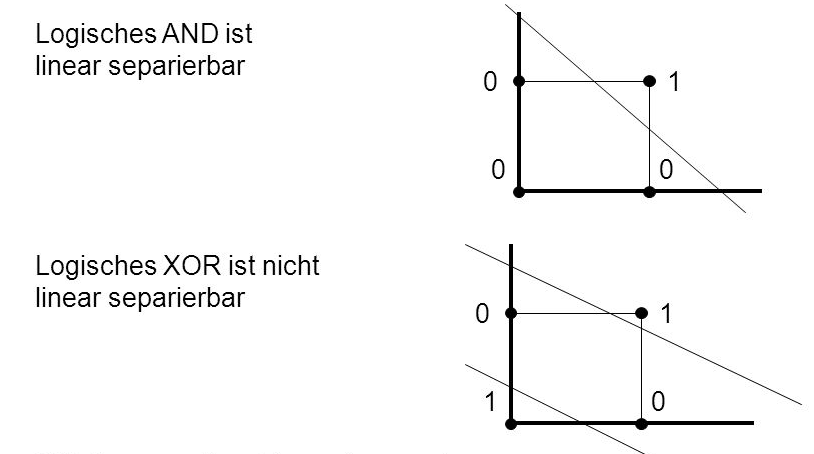
\includegraphics[width=0.71\textwidth]{Bilder/Konzeption/Linear_Sep.PNG}
	\caption{Bildliche Erläuterung der linearen Separierbarkeit}
	\label{fig:Bildliche Erläuterung der linearen Separierbarkeit}
\end{figure}

Analog setzt sich dies in Funktionen höherer Dimensionen fort. Ist die Funktion zum Beispiel dreidimensional, erfolgt die Separierung durch eine Ebene.

Nachdem der Begriff der linearen Separierbarkeit erläutert wurde, kann dies als Grundlage für den nächsten Schritt genutzt werden. Zur Auswahl des passenden Netztyps kann nun der Beweis 1 betrachtet werden. Dieser von Minski und Pappert erstellte Beweis  belegt, dass einschichtige KNN nur in der Lage sind, linear separierbare Funktionen zu berechnen.\footnote{\Vgl\Zitat{Laemmel}, Seite 212 f.}

\newpage

\newmdtheoremenv{bew}{Beweis}
\begin{bew}Beweis der eingeschränkten Fähigkeit von KNN anhand des XOR-Problems\\

Gegeben sind ein Perzeptron der folgenden Bauart

\begin{figure}[H]
\centering
		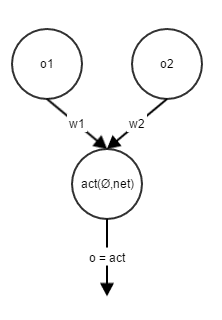
\includegraphics[width=0.30\textwidth]{Bilder/Konzeption/Perzeptron.PNG}
\end{figure}

sowie folgende Rahmenbedingungen:\\
$w_1\cdot o_1 + w_2\cdot o_2 = net$\\ 
$f_{act}(o) = id$ \\
$\emptyset = Schwellenwert$

Dann gilt:\\
$a) w_1\cdot 0 + w_2\cdot 0 < \emptyset$ Bei einem Inputvektor (0,0) liefert der Output 0.\\
$b) w_1\cdot 0 + w_2\cdot 1 \geq \emptyset$ Bei einem Inputvektor (0,1) liefert der Output 1.\\
$c) w_1\cdot 1 + w_2\cdot 0 \geq \emptyset$ Bei einem Inputvektor (1,0) liefert der Output 1.\\
$d) w_1\cdot 1 + w_2\cdot 1 < \emptyset$ Bei einem Inputvektor (1,1) liefert der Output 0.

Der Widerspruch ergibt sich wie folgt:\\ $(b+c): w_1 + w_2 \geq \emptyset  \wedge (d): w_1 + w_2 < \emptyset$
\end{bew}

Dieser Beweis kann ebenfalls auf andere nicht linear separierbare Funktionen angewandt werden. Somit steht fest, dass ein einschichtiges Perzeptron nicht in der Lage sein kann, nicht linear separierbare Funktionen zu approximieren.

Um festzustellen, ob eine Funktion linear separierbar ist, kann das Konvergenztheorem von Rosenblatt (Theorem 1) hinzugezogen werden\footnote{\Vgl\Zitat{Laemmel}, Seite 209}.

\newmdtheoremenv{theo}{Theorem}
\begin{theo}Konvergentheorem von Rosenblatt\\
Der Lernalgorithmus des Perzeptrons konvergiert in endlicher Zeit, d.h. das Perzeptron kann in endlicher Zeit alles lernen, was es repräsentieren kann.
\end{theo}

Es ergibt sich also folgende Relation:\\\\
Perzeptron konvergiert $\rightarrow$ Funktion linear separierbar $\rightarrow$ Perzeptron geeignet.
Und analog: Perzeptron konvergiert nicht $\rightarrow$ Funktion nicht linear separierbar $\rightarrow$ Perzeptron nicht geeignet.

Auf Basis der oben genannten Relation kann ermittelt werden, ob ein einschichtiges Perzeptron zur Approximation von Börsenkursen geeignet ist. Dafür wurde ein Perzeptron wie in Abbildung \ref{Testperz} entwickelt und untersucht, ob dieses Konvergiert.

\begin{figure}[H]
\hfill
\subfigure[Test-Perzeptron]{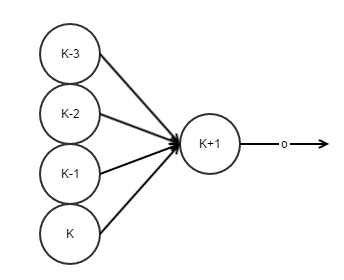
\includegraphics[width=7cm]{Bilder/Konzeption/Testperzeptron.PNG}}
\hfill
\subfigure[MSE des Perzeptrons]{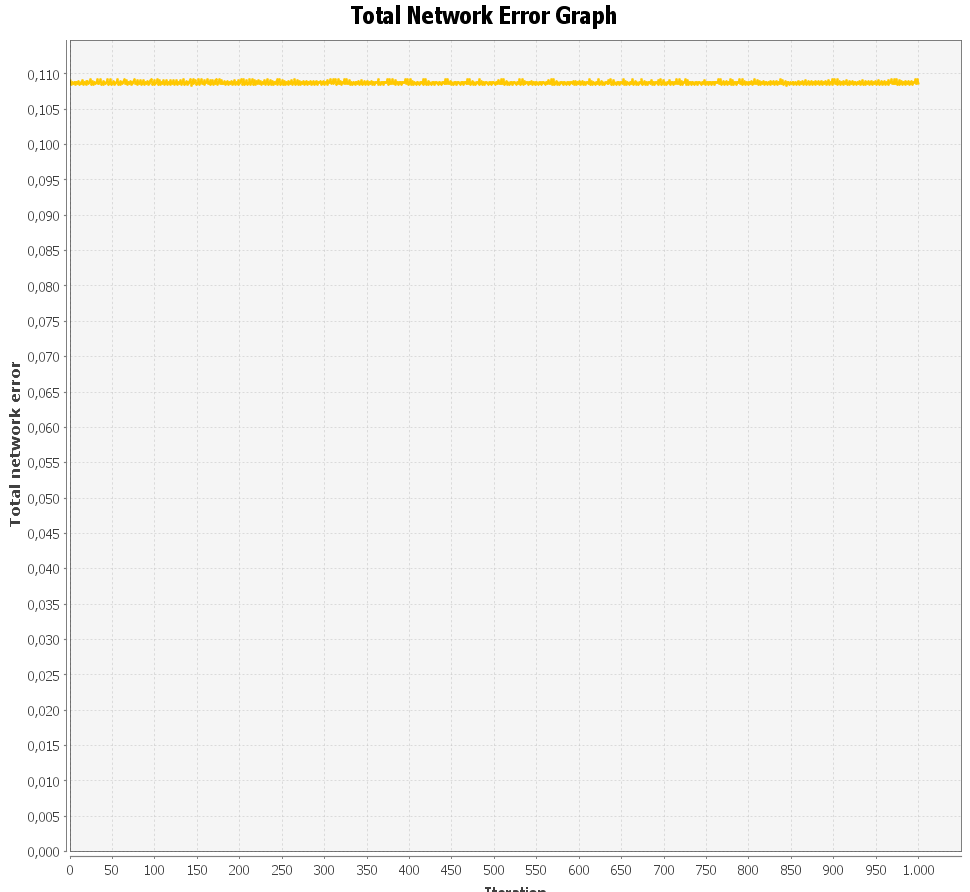
\includegraphics[width=7cm]{Bilder/Konzeption/MSEperzeptron.PNG}}
\hfill
\caption{Test-Perzeptron sowie der dazugehörige MSE}
\label{Testperz}
\end{figure}

Bei Betrachtung des Netzwerkfehlers des Perzeptrons erkennt man, dass das Perzeptron nicht konvergiert. Der Netzwerkfehler des Perzeptrons bleibt über alle Iterationen konstant auf einem Niveau von circa $0,10$. Somit steht fest, dass der Börsenkurs eine nicht linear separierbare Funktion darstellt und durch einen Perzeptron nicht approximiert werden kann.

Folglich bleibt nur noch das Multilayerperzeptron als Mögliche Auswahl übrig. Das dieses KNN tatsächlich zur Prognose geeignet ist, belegt das Theorem der universellen Approximation (Theorem 2)\footnote{\Vgl\Zitat{Cottbus}}.

\begin{theo}Theorem der universellen Approximation\\
Jede stetige Funktion kann mittels eines künstlichen neuronalen Netzes mit mindestens einer versteckten Schicht beliebig genau approximiert werden.
\end{theo}

Ein Börsenkurs kann prinzipiell jede beliebige (stetige) Funktion annehmen. Durch Theorem 2 ist jedoch sichergestellt, dass das Multilayerperzeptron in der Lage ist, diese Funktion zu approximieren, da ein Multilayerperzeptron als universeller Approximator fungiert.

\section{Wahl der Topologie}
\label{section:Wahl der Topologie}

Zur Prognose des Börsenkurses sollen die letzten vier Börsenkurse als Input dienen. Durch diesen Input soll der Börsenkurs am nächsten Tag prognostiziert werden. Folglich gestaltet sich Auswahl der Anzahl an Input-Neuronen (4) sowie Output-Neuronen (1) trivial.
Etwas komplexer gestaltet sich jedoch die richtige Dimensionierung der inneren Schicht. Hierbei können aber einige Richtlinien hinzugezogen werden, um die Dimensionierung zu erleichtern:

\begin{itemize}
\item Die Anzahl der versteckten Neuronen in der inneren Schicht sollte nicht zu groß gewählt werden, damit das Netz das antrainierte Verhalten nicht "`auswendig"' lernt. Sonst kann es nur das bereits trainierte Muster entsprechend verarbeiten. Dies bedeutet ein Verlust der Generalisierungsfähigkeit. Man spricht in diesem Fall von einem Overfitting.

\item Die Anzahl der versteckten Neuronen in der inneren Schicht sollte nicht zu klein gewählt werden, da eine gewisse Menge an Neuronen wichtig ist, um sich Regelsätze merken zu können.

\item Eine grobe Annäherung zur Bestimmung der Obergrenze der Anzahl von Neuronen in der versteckten Schicht liefert die folgende Formel\footnote{\Vgl\Zitat{Illmenau}}:

\begin{equation}\formelentry{Optimale Anzahl Neuronen in der versteckten Schicht}
  N_h = \frac{N_d}{10*(N_i+N_o)}
\end{equation}
$N_h$ ist hierbei die Obergrenze, $N_i$ die Anzahl der Input-Neuronen und $N_o$ die Anzahl der Output-Neuronen. Da $450$ Trainingsdaten verwendet werden sollen, bedeutet das für diese Seminararbeit konkret:

\begin{equation}\formelentry{Optimale Anzahl Neuronen in der versteckten Schicht}
  N_h = \frac{450}{10*(4+1) = 9 }   
\end{equation}
\end{itemize}
 
Somit ergibt sich insgesamt die folgende Topologie aus Abbildung \ref{fig:Grundlegende Topologie des KNN}. 

\begin{figure}[H]
\centering
		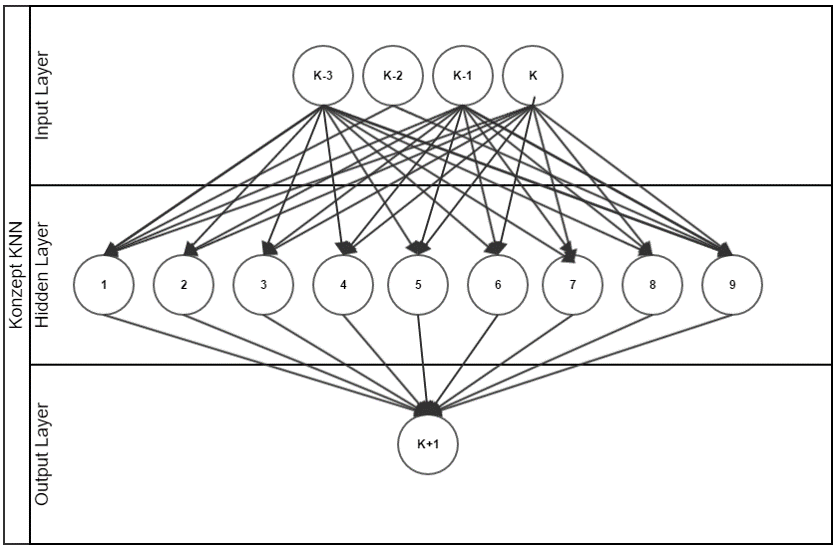
\includegraphics[width=0.75\textwidth]{Bilder/Konzeption/KonzKNN.PNG}
	\caption{Grundlegendes Konzept des KNN}
	\label{fig:Grundlegende Topologie des KNN}
\end{figure}

Dieses KNN stellt ein solides Grundkonstrukt dar, das in der Umsetzungsphase noch weiter optimiert werden kann.

\section{Wahl des Lernverfahrens} 
\label{section:Wahl des Lernverfahrens}

Grundsätzlich existieren drei Lernverfahren, wie ein KNN trainiert werden kann. In diesem Abschnitt werden alle drei Lernverfahren näher vorgestellt und anschließend eine begründete Auswahl des gewählten Verfahrens getroffen\footnote{\Vgl\Zitat{Laemmel}}.

\begin{itemize}
\item \textbf{Überwachtes Lernen}: \\
Beim überwachten Lernen sind sowohl die Eingabedaten als auch die dazugehörigen Ausgabedaten bekannt. Zunächst berechnet das KNN bestimmte Ausgabedaten zu den Eingabedaten. Diese berechneten Ausgabedaten können anschließend mit den tatsächlichen Ausgabedaten verglichen werden. Dieser Fehler wird dann genutzt, um die Verbindungsgewichte des KNN anzupassen. Typische Vertreter dieses Lernverfahrens sind die sogenannten Backpropagation-Lernverfahren.
	
\item \textbf{Bestärkendes Lernen}: \\
Ähnlich wie das überwachte Lernen, jedoch biologisch motivierter ist das sogenannte bestärkende Lernen. Hier sind dem KNN die Eingabewerte zwar bekannt, aber die dazugehörigen Ausgabewerte nur zum Teil oder gar nicht. Das KNN wird lediglich darüber informiert, ob das Ergebnis richtig bzw. falsch war. Es ist ein sehr zeitaufwändiges Lernverfahren, da es die Gewichte auf Grund der spärlichen Information nur sehr langsam anpassen kann. Dieses Verfahren kann als Mischung aus überwachtes Lernen und nicht überwachtes Lernen gesehen werden.

\item \textbf{Nicht überwachtes Lernen}: \\
Das nicht überwachte Lernen ist biologisch gesehen am plausibelsten. Bei diesem  Lernverfahren existieren nur Eingabemuster, jedoch keine erwünschten Ausgaben oder Angaben, ob das Netz die Eingaben richtig oder falsch klassifiziert hat. Stattdessen versucht der Lernalgorithmus selbständig, Gruppen ähnlicher Eingabevektoren zu identifizieren und diese auf Gruppen ähnlicher oder benachbarter Neuronen abzubilden. 
\end{itemize}

Da sowohl die Eingabewerte als auch die Ausgabewerte der zu verwendenden Datensätze bekannt sind, bietet sich das überwachte Lernen an. Verglichen mit den anderen Lernverfahren ist dies die effizienteste Lernmethode. Sie verfügt zwar über kein biologisches Vorbild, dieser Umstand hat aber für diese Seminararbeit keine Relevanz.
